\documentclass[oneside,12pt]{book}  % reqno mette i numeri a destra

\usepackage{moresize}  % serve per avere il fonte \HUGE
\usepackage{a4}  % per stampare in formato a4
\usepackage{amssymb,amsfonts,amsmath}  % serve per includere le macro pi`u potenti dell'AMS per le formule 
\usepackage{eucal,mathrsfs} % Per avere un calligrafico piu' bello
\usepackage[british,UKenglish,USenglish,english,american]{babel}  % per  gli a capo secondo le regole dell'italiano
\usepackage{graphicx} % serve per importare le figure in formato jpg, png, pdf
\usepackage{enumerate}  % Utile per creare items personalizzati
\usepackage{color} % Se vuoi usare i colori, altrimenti toglilo
%\usepackage[
%color,
%draft]        % per togliere showkeys sostituire draft con final
%{showkeys}    % molto utile per stampare i nomi che hai dato alle varie label, compaiono nel draft. Nella versione finale 
%                      basta mettere final oppure commentare l'istruzione per togliere le label.
%% 
\usepackage{pdfsync} % molto utile per saltare dal testo al pdf e vicevera.
%%% MIEI
\usepackage{subfigure}
\usepackage{amsmath}
\usepackage{amsthm}
\usepackage[applemac]{inputenc}
\usepackage{listings} 
\usepackage{placeins}


\theoremstyle{plain} 
\newtheorem{thm}{Teorema}[section] 
\newtheorem{cor}[thm]{Corollario} 
\newtheorem{lem}[thm]{Lemma} 
\newtheorem{prop}[thm]{Proposizione} 

\theoremstyle{definition} 
\newtheorem{defn}{Definizione}[chapter] 

\theoremstyle{remark} 
\newtheorem{oss}{Osservazione} 

%%
%%
%%
%%
\newtheorem{teorema}{Teorema}[chapter]  % per cambiare la numerazione
                                        % basta mettere chapter 
\newtheorem{lemma}[teorema]{Lemma}
\newtheorem{corollario}[teorema]{Corollario}
\newtheorem{proposizione}[teorema]{Proposizione}
\newtheorem{osservazione}[teorema]{Osservazione}
\newtheorem{esempio}[teorema]{Esempio}
\newtheorem{definizione}[teorema]{Definizione}
\newtheorem{problema}[teorema]{Problema}
\newtheorem{ipotesi}[teorema]{Ipotesi}
%%
\numberwithin{equation}{chapter} % serve per numerare le formule in accordo ai capitoli.
%%
%% ALTRE MACRO: nel file macro.tex ho messo tutte le macro che sono utili per i vari simboli. Vengono incluse dall'istruzione
%%
\input macro
%%
%% Se non ti servono (ma sono utili) commenta l'input
%%
%%
%%%%%%%%%%%%%%%%%%%%%%%%%%%%%%%%%%%%%%%%%%%%%%%%%%%%%%%%%%%%%%%%%%%%%%%%%%%%
%%
%%                   TITOLO, INDICE
%%
%%%%%%%%%%%%%%%%%%%%%%%%%%%%%%%%%%%%%%%%%%%%%%%%%%%%%%%%%%%%%%%%%%%%%%%%%%%%
%%
%%
\makeindex % serve se vuoi fare un indice delle parole alla fine; altrimenti commenta.
\begin{document}

% Code package
\lstset{language=Matlab} 

\thispagestyle{empty}  % toglie il numero di pagina alla pagina inziale
\begin{center}  % serve per centrare un testo  
  {\Large Politecnico di Milano}\\[12pt]    % serve  per andare a capo lasciando uno spazio voluto.

  {\Huge Progetto di \\
  Numerical Analysis for Partial Differential Equations\\
  e Advanced Programming for Scientific Computing }
\end{center}


\begin{center}    % qui metti il titolo della tesi
  \Huge \bf Virtual Element Method
\end{center}
%
\vspace{12pt}
%
\begin{flushleft}
  \noindent\Large
  Students:\\
  Nicolo\`o Ripamonti \\
  Stefano Savar\`e\\
  
\end{flushleft}
%
% \begin{flushright}
%   \noindent\LARGE
%   Tesi di Laurea di:\\
%   Stefano Savar\`e - Matr.
% \end{flushright}
%
\vspace{364pt}
%
\begin{center}
  \large
  Anno Accademico 2014-2015
\end{center}

\newpage

\tableofcontents  %serve per creare l'indice iniziale

%%
%%
%%%%%%%%%%%%%%%%%%%%%%%%%%%%%%%%%%%%%%%%%%%%%%%%%%%%%%%%%%%%%%%%%%%%%%%%%%%%
%%
%%                   INIZIO DELLA TESI
%%
%%%%%%%%%%%%%%%%%%%%%%%%%%%%%%%%%%%%%%%%%%%%%%%%%%%%%%%%%%%%%%%%%%%%%%%%%%%%

% \part{NOME}    % se devi dividere la tesi in piu parti


\renewcommand{\baselinestretch}{1.5} % se vuoi aumentare l'interlinea; altrimenti commenta.

% istruzioni per le sezioni: \chapter{}, \chapter*{}, \section, \section*
% l'asterisco non mette il numero
%%
 
\addcontentsline{toc}{chapter}{Introduction}  % serve per creare la voce Introduzione nella table of contents iniziale

\chapter{Algoritmi utilizzati}
\label{ch:algorithms}
In questo capitolo diamo una descrizione teorica degli algoritmi che
abbiamo usato per determinare alcune specifiche propriet\`a degli
elementi della mesh. Nel caso degli Elementi Finiti, determinare
quantit\`a come l'area o la normale esterna a un poligono, non \`e un
compito complesso in quanto \`e necessario gestire solo elementi
triangolari.
Una delle caratteristiche principali dei VEM, invece, \`e la
possibilit\`a di trattare mesh di poligoni/poliedri qualunque, anche concavi:
la complessit\`a dell'operazione \`e dunque molto aumentata.

Non avendo trovato in letteratura un articolo unico che parlasse
contemporaneamente di tutti questi problemi, proponiamo qui gli
algoritmi principali da noi utilizzati. La maggior parte sono stati
trovati on-line, ad alcuni abbiamo apportato nostre modifiche per
adattarli al nostro caso.

\section{Poligoni}
Un poligono nella nostra implementazione \`e definito come un insieme
\textit{ordinato} di punti. 
\`E necessario calcolare:
\begin{itemize}
\item Area
\item Normale orientata
\item Baricentro
\end{itemize}
Per ciascuno di questi \`e necessario fornire un'implementazione
differente nel caso il poligono sia in 2D o sia immerso in uno spazio 3D.

\subsection{Area in 2D}
Si \`e sfruttata la formula dell'area di Gauss-Green:

$$ A=\frac{1}{2} \bigg | \sum_{i=1}^n (x_iy_{i+1}-x_{i+1}y_i) \bigg
|$$
dove si \`e usata la convenzione $x_{n+1},y_{n+1}=x_1,y_1$

% \begin{proof}
% Si consideri la forma differenziale $$ \omega=\frac{x dy}{2}-\frac{y
%   dy}{2}$$.
% Per il teorema di Green si ha: $$ \int_\Omega d\omega = \int_{\partial
% \Omega} \omega = \sum^n_{i=1}\int_{A(i)}\omega =
% \frac{1}{2}\sum_{i=1}^n \int_{A(i)}x dy-y dx$$,
% dove $A(i)$ \`e il segmento che unisce il punto $(x_i,y_i)$ a
% $(x_{i+1},y_{i+1})$.
% Attraverso una parametrizzazione ottengo:
% $$\frac{1}{2}\sum_{i=1}^n
% \int_0^1(x_i+(x_{i+1}-x_i)t)(y_{i+1}-y_i)-(y_i+(y_{i+1}-y_i)t)(x_{i+1}-x_i)dt$$,
% e integrando
% $$\frac{1}{2}\sum_{i=1}^n
% \frac{1}{2}[(x_i+x_{i+1})(y_{i+1}-y_i)-(y_i+y_{i+1})(x_{i+1}-x_i)]$$
% Svolgendo i calcoli ottengo la tesi:
% $$\frac{1}{2} \sum_{i=1}^n (x_iy_{i+1}-x_{i+1}y_i) $$

% \end{proof}

\subsection{Area in 3D}
Per il caso 3D abbiamo usato un algoritmo simile. L'algoritmo usato
\`e il seguente:
\begin{enumerate}
\item Proietto il poligono su uno dei tre piani principali $xy$, $xz$,
  $yz$. 
Dato un vertice $(x,y,z)$ pongo a 0 la componente corrispondente al
massimo indice della normale al poligono. In questo modo ottengo
l'equivalente di un poligono 2D. Eliminando la componende con indice
maggiore si evita il caso di poligono gi\`a parallelo ad uno dei tre
piani. In questo caso infatti la proiezione risulterebbe in un
poligono degenere.

\item Calcolo l'area del poligono proiettato con la formula dell'area
  di Gauss

\item Divido per un apposito scale factor. Tale valore \`e calcolato
  come:
$$ \frac{\max_i (\nn[i])}{||\nn||} $$,
dove $\nn$ \`e la normale al poligono.

\end{enumerate}

\subsection{Normale orientata}
Attraverso la nostra definizione di poligono, avendo gi\`a un
ordinamento tra i punti, il verso della normale
\`e ottenuto attraverso la regola della mano destra.
Tale calcolo per un poligono concavo non \`e
elementare. Sarebbe invece pi\`u semplice calcolare la semplice
direzione.
Sfruttando l'algoritmo di Newell, nel caso di poligono immerso in 3D
la normale \`e ottenuta con la seguente formula:

$$
\begin{cases}
N_x=\sum_{i=0}^{n} (y_i-y_{i+1})(z_i+z_{i+1}) \\
N_y=\sum_{i=0}^{n} (z_i-z_{i+1})(x_i+x_{i+1}) \\
N_z=\sum_{i=0}^{n} (x_i-x_{i+1})(y_i+y_{i+1}) 
\end{cases}
$$

Nel caso 2D l'algoritmo \`e il medesimo, ma non vengono pi\`u
calcolate le componenti $N_x$ e $N_y$ che sono 0.

\subsection{Baricentro}
Nel caso 2D la formula per calcolare il baricentro $C$ di un poligono
\`e la seguente:
$$
\begin{cases}
C_x=\frac{1}{6A}\sum_{i=0}^{n} (x_i+x_{i+1})(x_iy_{i+1}-x_{i+1}y_i) \\
C_y=\frac{1}{6A}\sum_{i=0}^{n} (y_i+y_{i+1})(x_iy_{i+1}-x_{i+1}y_i) \\
\end{cases}
$$
dove $A$ \`e l'area con segno del poligono, data dalla formula:
$$A=\frac{1}{2} \sum_{i=1}^n (x_iy_{i+1}-x_{i+1}y_i) $$
Il caso 3D \`e implementato in modo simile, l'algoritmo \`e il
seguente:

\begin{enumerate}
\item Se il poligono giace su un piano parallelo a $xy$, $xz$ o
  $yz$ l'algoritmo \`e identico al caso 2D

\item Altrimenti viene dapprima proiettato su uno dei tre piani, come
  per l'algoritmo per determinare l'area, e
 procedendo come nel caso 2D vengono determinate 2 delle 3
  componenti del baricentro. Viene successivamente proiettato su un
  altro dei 3 piani per determinare l'ultima componente.

\end{enumerate}


\section{Poliedri}
Un poliedro nella nostra implementazione \`e definito come un insieme
\textit{non ordinato} di poligoni.
Diversamente dal caso poligonale non abbiamo implementato un algoritmo
esatto per il calcolo del baricentro. Tale valore non \`e necessario
per il nostro progetto e richiede un alto costo computazionale.
\`E invece necessario determinare:
\begin{itemize}
\item Volume
\item Orientamento coerente della normale tra le facce di un poliedro
\item Determinare se la normale \`e esterna o interna
\end{itemize}

\subsection{Volume}
Per il volume si \`e sfruttato il teorema della divergenza: sfruttando
la relazione:
$$ \int_\Omega \nabla \cdot \FF d\omega=\int_{\partial\omega}\FF \cdot
\nn ds $$
ponendo $$\FF=x$$ ottengo:
$$ \int_\Omega d\omega=\int_{\partial\omega} \xx \cdot \nn ds =\int_{\partial\omega} x  n_x ds $$
Il secondo integrale pu\`o essere scomposto in integrale su ogni
faccia del poliedro:
$$ \int_{\partial\omega} x n_x ds=\sum_{i=1}^k \int_{A_i} x n_x ds$$
dove $k$ \`e il numero di facce del poliedro e $A_i$ \`e la faccia.
Si noti che
$$\int_{A_i} x n_x ds= |A_i| n_x  \bar x_i $$
dove $|A_i|$ \`e l'area del poligono $A_i$ e $\bar x_i$ \`e la
componente $x$ del baricentro di $A_i$.
Ottengo dunque:
$$ V= \sum_{i=1}^k |A_i|  n_x \bar x_i $$
Conoscendo area, baricentro e normale delle facce la formula \`e dunque di
veloce implementazione.
 
\subsection{Orientamento della normale coerente tra le facce}
Scopo di questo algoritmo \`e di far si che, dato un poliedro, le
facce siano orientate coerentemente, ossia che la
normale sia, per tutte le facce, o interna o esterna al poliedro. L'algoritmo \`e il seguente:

\begin{enumerate}
\item Fornisci un ordinamento tra le facce del poliedro.
\item Per ciascuna faccia controlla per tutte le successive
  nell'ordinamento se hanno lati in comune.
\item Se si, se il lato compare in ordine opposto nelle due facce
  l'orientamento \`e coerente (la normale dei due poligoni punta per
  entrambi o verso l'esterno o verso l'interno). Altrimenti inverti l'ordine dei vertici
  nella seconda faccia per ottenere un orientamento coerente. Modifica l'ordinamento delle facce,
  posizionando la seconda faccia davanti a quella
  di partenza.

\item Se no continua senza ulteriori operazioni.

\item Una volta controllate tutte le facce successive nell'ordinamento
  continua con la prima faccia nell'ordinamento non ancora controllata.

\end{enumerate}

\subsection{Determinare se la normale \`e esterna o interna}
Una volta ottenuto un ordinamento coerente tra le facce del poliedro,
\`e necessario ordinarle tutte verso l'esterno, per calcolare
correttamente i termini di bordo nei metodi numerici.

L'algoritmo da noi implementato \`e una versione 3D del \textit{Ray
  casting algorithm}. Questo in 2D consiste nel determinare se un
punto \`e esterno o interno ad un poligono. Per ottenere questa
informazione si conta il numero di intersezioni di un raggio
proveniente dall'esterno e diretto verso tale punto. Se questo numero \`e pari il
punto \`e esterno, se dispari il punto \`e interno. Pu\`o essere
riproposto in modo pressoch\`e identico nel caso 3D, anche se con un
costo computazionale elevato.

Una problematica nel caso 2D che si ripropone anche in quello 3D \`e
il caso in cui l'intersezione del raggio con il poligono avviene in un
vertice invece che in un lato. In questo caso per ottenere un
risultato corretto \`e necessario modificare il raggio considerato. 

Poich\`e tutte le facce sono orientate coerentemente \`e sufficiente
orientare correttamente la normale ad un unica faccia e nel caso di
modifiche invertire il verso di tutte le altre facce.
L'algoritmo da noi proposto \`e il seguente:
\begin{enumerate}
\item Considera la prima faccia del poliedro e un punto scelto
  casualmente su di essa.
\item Considera il prolungamento della normale avente origine in tale
  punto.
\item Se tale prolungamento interseca un vertice o uno spigolo del poliedro
  seleziona un altro punto casualmente e ripeti il procedimento
\item Conta il numero di intersezioni con le facce del poliedro di
  tale semiretta. Questo punto \`e quello pi\`u costoso computazionalmente.
\item Se pari la normale \`e esterna, se dispari la normale \`e
  interna.
\item Se interna inverti l'orientamento di tutte le facce del poliedro
  per averla esterna.

\end{enumerate}



 

\chapter{Implementazione}
\label{ch:implementazione}

Scopo della parte implementativa del progetto \`e creare un codice che consenta di risolvere
il problema di Laplace con condizioni al bordo di Dirichlet in 2D o 3D
su mesh composte rispettivamente da generici poligoni e poliedri.
Descriviamo in questo capitolo il codice da noi sviluppato. Abbiamo
utilizzato il linguaggio C++, secondo la logica della programmazione
ad oggetti. Attraverso un semplice Makefile \`e possibile automatizzare la
compilazione e sfruttando Doxygen viene generata automaticamente la
documentazione del codice.
Per la parte di visualizzazione del codice abbiamo invece preferito
creare alcuni script Python, sfruttando la libreria Mayavi per i
grafici 3D.
Abbiamo utilizzato uno stile di codice il pi\`u possibile coerente per
facilitarne la comprensione.

\section{Panoramica del codice}
\label{sec:panoramica}
Il codice \`e basato su 18 classi e un file main. Sfruttando le
tecniche del \textit{template programming}, dichiarazione e
implementazione delle classi sono entrambe nel file header.
La gestione della memoria \`e stata effettuata con le pi\`u recenti
tecniche del C++11 allo scopo di evitare memory leak: in particolare i puntatori,
dove necessari, sono stati implementati come shared pointers o weak
pointers.
Scopo dell'implementazione \`e stato il creare un codice il pi\`u
possibile generale e riutilizzabile. 
Il lavoro \`e diviso idealmente in due parti principali:
\begin{itemize}
\item
\textbf{La mesh:} 7 classi con cui viene modellizzata una qualunque
Mesh 2D o 3D formata da elementi non convessi in generale. La
possibilit\`a nei VEM di trattare figure qualunque ha
reso questa parte piuttosto articolata e computazionalmente non
trascurabile. Il calcolo di specifiche propriet\`a dei
poligoni/poliedri (es. volume, normale esterna) \`e significativamente
pi\`u complesso che nel caso standard, ma nondimeno indispensabile per
la risoluzione del problema.

\item
\textbf{La risoluzione del problema con i VEM:} in questa parte si \`e
cercato dapprima di creare un codice che consenta di risolvere il
problema di Laplace su una mesh qualsiasi a prescindere dal tipo di
solver e dalle condizioni al bordo. Dopo di ch\'e si \`e implementato
il solver per il Virtual Element Method e le condizioni al bordo di
Dirichlet, le uniche trattate in questo progetto.
L'idea di base dell'implementazione di questa parte \`e stata di
creare un codice sufficientemente generale da consentire di modificare
il metodo utilizzato (ad esempio FEM al posto che VEM) semplicemente
scrivendo la parte relativa al solver e non quella relativa al
problema o alle condizioni al bordo.
\end{itemize}
A queste due parti principali si aggiunge il file \textit{main}, in
cui viene lanciato il solutore appropriato in base ad alcuni parametri
presenti in un \textit{datafile}. Questo per evitare di dover
ricompilare il programma ad ogni piccola modifica.

Come gi\`a detto vi \`e poi una parte separata di codice, scritto questa
volta in Python, destinato alla visualizzazione grafica. Si \`e scelto
questo linguaggio per la sua semplicit\`a rispetto al C++ e per la
presenza di una libreria, \textit{Mayavi}, adatta alla visualizzazione
3D. Questa parte \`e intesa come completamento della precedente,
scritta allo scopo di fornire un modo rapido di testare graficamente
la soluzione.

\section{La Mesh}
\label{sec:mesh}
Abbiamo scelto di scrivere da zero il codice per la Mesh per via delle
particolarit\`a dei VEM che richiedono elementi pi\`u generali che nel
classico caso degli Elementi Finiti. 

La Mesh in 3 dimensioni \`e stata pensata come un insieme di
poliedri. Ciascuno di questi \`e a sua volta composto da un insieme di
poligoni che a loro volta sono definiti come insieme ordinato
di punti. Le 3 classi che rappresentano poliedri, poligoni e punti
sono quelle su cui si \`e basata la costruzione della mesh; sono
estremamente interconnesse tra loro: ciascun poliedro contiene
un vettore di puntatori ai vertici e alle facce dello stesso e viceversa. Questo
comporta alcune difficolt\`a nel costruttore, che sono state superate
con la tecnica dei variadic template e un metodo dedicato
esplicitamente alla creazione di un'istanza. Per i puntatori come
gi\`a detto abbiamo usato gli \textit{shared\_pointer} per facilitare
la gestione della memoria. 
Non abbiamo usato i pi\`u efficienti \textit{unique\_pointers}
in quanto all'interno del programma lo stesso puntatore \`e condiviso
da pi\`u classi.
Il caso 2D \`e implementato in modo analogo salvo l'assenza dei
poliedri. Non si \`e rivelata invece necessaria una classe Edge, non
\`e stata dunque implementata ai fini di rendere pi\`u semplice la struttura.

Tratto comune a tutte le classi
\`e la presenza di due parametri template, \textit{embedded} e
\textit{real}, che garantiscono flessibilit\`a dal punto di vista
dello spazio scelto (2D o 3D) e della precisione dei numeri a virgola
mobile (double o long double). 

\subsection{Point e MeshPoint}
Queste 2 classi rappresentano un punto in uno spazio di una
specificata dimensione. La differenza tra le due \`e che la prima \`e
intesa per un punto generico, la seconda per un punto appartenente ad
una mesh. Quest'ultima memorizza al suo interno anche i poligoni e i
poliedri che hanno tale punto come vertice e non \`e stato fornito un
copy constructor. Ha inoltre la possibilit\`a di tener traccia dell'ID
del punto e se tale punto \`e sulla frontiera.

La classe Point viene utilizzata anche per rappresentare un vettore,
sono quindi stati forniti i metodi opportuni, come il calcolo della
norma e il prodotto vettore. 

La presenza o meno del copy constructor \`e la maggiore differenza tra
le due classi: nella classe Point \`e molto utile per velocizzare
diverse operazioni, in MeshPoint invece \`e addirittuara dannoso, in
quanto, data la stretta interconnessione tra le classi che formano la
mesh, copiare uno dei suoi elementi renderebbe molto difficile
preservare correttamente tali collegamenti.

\noindent\rule{14cm}{1pt}

Riportiamo qui l'interfaccia della classe Point e i metodi principali:

\begin{verbatim}
template <long embedded,typename real=double>
class Point {

protected:
    array<real,embedded> coordinates;

public:
    // CONSTRUCTORS
    Point(const array<real,embedded>& inputArray);
    Point(const Point<embedded,real>& inputPoint);
    Point(const MeshPoint<embedded,real>& inputPoint);

    // Constructor with variadic template
    template <typename... Args>
    Point(Args... arguments);

    // STANDARD METHOS
    long maxIndex() const;	//!< Maximum index of the point
    long maxAbsIndex() const;	//!< Maximum index of the point with absolute value
    real norm() const;  //!< L2 norm of the vector
    real normL1() const; //!< L1 norm of the vector

    real& operator[](long index);	//!< Get an element by
reference

    template <long embedded2,typename real2>
    friend Point<embedded2,real2> cross(const Point<embedded2,real2>&
point1, const Point<embedded2,real2>& point2);
\end{verbatim}

\noindent\rule{14cm}{1pt}

Riportiamo l'interfaccia della classe MeshPoint e i metodi principali:

\begin{verbatim}
template <long embedded,typename real=double>
class MeshPoint: public Point<embedded,real> {
protected:
    // PROPERTIES
    long pointID;	//!< ID of the MeshPoint
    real value;		//!< Value in the point after the resolution of the problem
    bool isBoundary;	//<! Tells if the MeshPoint is on the boundary

    vector<weak_ptr<Polygon<embedded, real>>> polygonVector;
    vector<weak_ptr<Polyhedron<embedded,real>>> polyhedronVector;

    // CONSTRUCTORS
    // Constructor with variadic template
    template <typename... Args>
    MeshPoint(Args... arguments);

    // STANDARD METHODS
    void addPolygon(weak_ptr<Polygon<embedded,real>> inputPolygon); 
//!< It insert in polygon vector a new Polygon
    void addPolyhedron(weak_ptr<Polyhedron<embedded,real>> inputPolyhedron);	
//!< It insert in polyhedron vector a new Polyhedron


\end{verbatim}

\subsection{Polygon e Polyhedron}
Queste due classi rappresentano un poligono o un poliedro generico,
non convesso in generale. Entrambi sono da intendersi come componenti
di una mesh, non sono state realizzate due versioni come per point in
quanto non necessarie. Valgono dunque le stesse considerazioni
sull'assenza di copy constructor proposte per MeshPoint.
Per entrambe l'unico modo per creare una nuova
classe \`e sfruttando il metodo \textit{make\_shared\_Polygon} o
\textit{make\_shared\_Polyhedron}, che restituisce uno shared pointer
all'oggetto e si occupa anche di gestire le connessioni tra
essi. L'utilizzo della tecnica dei \textit{variadic template}
garantisce una certa flessibilit\`a e leggibilit\`a nel codice. Ad
esempio un \textit{Polygon} pu\`o essere inizializzato sia da un
\textit{std::vector} di \textit{MeshPoint}, sia da una sequenza di
lunghezza arbitraria degli stessi.

Polygon \`e da intendersi come un vettore \textit{ordinato} di Point,
pu\`o essere sia in 2D che in 3D. L'ordinamento dei punti \`e necessario
sia per il fatto che non \`e possibile individuare un poligono non
convesso da un insieme non ordinato di punti, sia per determinare il
verso della normale. In fase di inizializzazione vengono calcolate le
seguenti quantit\`a, necessarie per il problema numerico:
\begin{itemize}
\item area
\item normale
\item baricentro
\end{itemize}

 Polyhedron invece \`e un vettore \textit{non ordinato} di Polygon. 
In fase di inizializzazione vengono calcolate le seguenti quantit\`a, 
necessarie per il problema numerico:
\begin{itemize}
\item volume 
\item normale esterna
\item baricentro
\end{itemize}
Fa inoltre in modo che le normali delle facce siano orientate
coerentemente. Gli algoritmi utilizzati per calcolare queste
quantit\`a sono proposti nel capitolo \ref{ch:algorithms}.

\noindent\rule{14cm}{1pt}

Riportiamo l'interfaccia della classe Polygon e i metodi principali:

\begin{verbatim}
template <long embedded, typename real=double>
class Polygon: public std::enable_shared_from_this<Polygon<embedded,real>> {
protected:
    // PROPERTIES
    // Vector of ordered vertexes
    vector<shared_ptr<MeshPoint<embedded,real>>> pointVector;
	
    bool isBoundary;	// Tells if the Polygon is on the boundary
    real area;	// \return the area of the Polygon
    Vector<3, real> normal;	// oriented normal to the Polygon
    Point<embedded, real> centroid;	// centroid of the Polygon
    vector<weak_ptr<Polyhedron<embedded,real>>> polyhedronVector;

public:
    // CONSTRUCTORS
    Polygon(const privateStruct &,
const vector<shared_ptr<MeshPoint<embedded,real>>>& vertexVector);
    // Constructor with variadic template.
    template <typename... Args>
    Polygon(const privateStruct&,Args... arguments);

    template <typename... Args>
    static shared_ptr<Polygon<embedded,real>> make_shared_Polygon(Args... arguments);

public:
    // STANDARD METHODS
    // Add a new vertex to the Polygon
    void addPoint(const shared_ptr<MeshPoint<embedded,real>>& p1); 
    // Add a new Polyhedron having this as face
    void addPolyhedron(weak_ptr<Polyhedron<embedded,real>> polyhedron);	
			
    Vector<embedded,real> computeCentroid();
    real computeArea();
    real getDiameter();
    real hTriangle(); // Compute the maximum distance between 2 vertexes.

    shared_ptr<MeshPoint<embedded,real>> isPointAVertex(Point<embedded,real>& point);	
    bool isPointInside(Point<embedded,real>& point);
    array<shared_ptr<MeshPoint<embedded,real>>,2> 
isPointOnBoundary(Point<embedded,real>& point);

    Vector<3,real> computeNormal();
    void switchPointsOrder(); // Invert the orientation of the Polygon

\end{verbatim}

\noindent\rule{14cm}{1pt}

Riportiamo l'interfaccia della classe Polyhedron e i metodi principali:

\begin{verbatim}
template <long embedded, typename real=double>
class Polyhedron: public enable_shared_from_this<Polyhedron<embedded,real>> {

protected:
    // PROPERTIES
    // Stores the faces of the Polyhedron
    vector<shared_ptr<Polygon<embedded,real>>> polygonVector; 
	
    bool isBoundary;	// Tells if the Polygon is on the boundary
    real volume;	// volume of the Polyhedron
    Point<embedded,real> centroid;	// Not the real centroid, 
only the mean of the vertexes.

    // Stores the vertexes of the Polyhedron
    vector<shared_ptr<MeshPoint<embedded,real>>> pointVector;	

public:
    // CONSTRUCTORS
    Polyhedron(const privateStruct&,
const vector<shared_ptr<Polygon<embedded,real>>>& inputPolygonVector);
    // Constructor with variadic template. DO NOT USE.
    template <typename... Args>
    Polyhedron(const privateStruct&,Args... arguments)

    template <typename ...Args>
    static shared_ptr<Polyhedron<embedded, real>>
make_shared_Polyhedron;

    // STANDARD METHODS
    // Add a new vertex to the Polygon
    void addPolygon(shared_ptr<Polygon<embedded,real>>& inputPolygon);
    // Add a new Polyhedron having this as face
    void addPoint(shared_ptr<MeshPoint<embedded,real>>& inputPoint);
    Point<embedded,real> computeCentroid();	// return the centroid
    real computeVolume();	// return the volume of the Polyhedron
    real getDiameter();		// return the maximum distance between 2 Points
    // Makes the normal to each face pointing towards the external of the Polyhedron
    void fixExternalNormal();	
    // Makes the normal of each face pointing in the same direction (or inward or outward)
    void fixFacesOrientation();	
    // Maximum distance between vertexes. Necessary for the mesh.
    real hTriangle();	
    void linkPoints();	// Makes all vertexes pointing to this
    void linkPolygons();  // Makes all Polygons pointing to this

    void switchFacesOrientation();	// Invert the orientation of all faces
    // If a new face is added, also his vertexes are added to the pointVector
    void updatePointVector();	


\end{verbatim}

\subsection{Mesh, Mesh2D e Mesh3D}
Mesh \`e una classe astratta che ha lo scopo di rappresentare
una mesh molto generica (anche ad esempio una superficie in uno spazio
3D). L'idea alla base \`e di memorizzare due vettori, uno di Point e
uno di Polygon o Polyhedron a seconda dello spazio scelto, e di creare
dei metodi base per la lettura di diverse tipologie di file, che poi
verranno implementati opportunamente nelle classi derivate. Sono
presenti anche 2 appositi metodi virtuali per tener traccia degli elementi alla
frontiera e per settare eventualmente altre propriet\`a della mesh. Non \`e
stato implementato un costruttore, ma viene fornito un metodo
\textit{initialize} che pu\`o essere chiamato dal costruttore di una
classe derivata per l'inizializzazione.

Mesh2D \`e la classe derivata di Mesh per gestire mesh in 2
dimensioni. Per il rilevamento degli elementi di frontiera si sono
cercati i lati presenti in un solo poligono nella mesh. Per
velocizzare la ricerca e dal momento che non \`e presente una classe
Edge, \`e stato introdotto un vettore di coppie di punti, denominato
\textit{pairVector}, evitando cos\`i la creazione di un'apposita
classe Edge che avrebbe reso il codice inutilmente pi\`u complesso.
Una volta creata la mesh il \textit{pairVector} viene analizzato per
trovare lati non duplicati.


Mesh3D \`e l'analogo nel caso tridimensionale. Per la maggiore
complessit\`a della mesh abbiamo ritenuto opportuno salvare in un
vettore anche i puntatori alle facce dei poligoni. Questo ci ha permesso di
ottenere gli elementi di frontiera con un algoritmo simile a quello
del caso 2D, ma confrontando le facce al posto dei lati. In questo
caso l'algoritmo di confronto viene chiamato direttamente all'inizializzazione di ogni nuova
faccia in quanto pi\`u veloce.

\noindent\rule{14cm}{1pt}

Riportiamo l'interfaccia della classe Mesh e i metodi principali:

\begin{verbatim}

template <long embedded,typename baseElement,OpenEnum isOpen=OPEN,
typename real=double>
class Mesh {
protected:
    
    // Vector of Polygon or Polyhedron
    vector<shared_ptr<baseElement>> elementVector;	
    // Vector of the vertexes of each element
    vector<shared_ptr<MeshPoint<embedded,real>>> pointVector;	
	
public:
    long numberOfElements;
    long numberOfPoints;

    virtual real hTriangle();	// paramether h of the Mesh
	
    // Method that calls the functions that read the file
    void initialize(string pointFile,string connection,MeshType meshType=ANYTHING3D);

    // It obtains the pointVector from file
    virtual void setPointVector(string file);	
    // It obtains the elementVector from connections
    virtual void setElementVector(string connections, MeshType meshType);
    
    // Virtual method to keep into account the boundary elements
    virtual void setBoundaryElements()=0;
    //	Virtual method used to set other things, like pointIDs
    virtual void setRemainingThings()=0;

    // methods to set the elementVector
    virtual void setTetrahedronMesh(string connection); 
    virtual void setTriangleMesh(string connection);	
    virtual void setAnything3DMesh(string connection);
    virtual void setAnything2DMesh(string connection);
    virtual void setFileType1Mesh(string connection);
    virtual void setFileType2Mesh(string connection);

    virtual void sort(); //!< Sort the pointVector based on pointID


\end{verbatim}

\noindent\rule{14cm}{1pt}

Riportiamo l'interfaccia della classe Mesh2D e i metodi principali:

\begin{verbatim}
template <typename real=double>
class Mesh2D: public Mesh<2,Polygon<2,real>,OPEN,real> {
private:
    // This is to obtain internal and external points	
    vector<pair<long,long>> pairVector;

public:
    long numberOfBoundaryPoints;
	
    // Constructor with input file
    Mesh2D(string pointFile,string connectionFile,MeshType meshType=ANYTHING2D);

    template <typename... Args >
    shared_ptr<Polygon<2,real>> newPolygon(Args... arguments);

    // Mesh of ANYTHING2D type
    virtual void setAnything2DMesh(string connection);

    virtual void setBoundaryElements();
    virtual void setRemainingThings();
\end{verbatim}

\noindent\rule{14cm}{1pt}

Riportiamo l'interfaccia della classe Mesh3D e i metodi principali:

\begin{verbatim}
template <typename real=double>
class Mesh3D : public Mesh<3, Polyhedron<3,real>, OPEN, real> {
protected:
    // Vector of all the Polyhedron faces
    vector<shared_ptr<Polygon<3,real>>> polygonVector;  

public:
    long numberOfPolygons;
    long numberOfBoundaryPoints;

    // Constructor with input file
    Mesh3D(string pointFile,string connectionFile,MeshType meshType=ANYTHING3D);
	
    // STANDARD METHODS
    // Method to create a Polygon after having read it.
    template <typename... Args >
    shared_ptr<Polygon<3,real>> newFace(Args... arguments);

    virtual void setBoundaryElements();
    virtual void setRemainingThings();

    // Mesh of TETRAHEDRON type
    virtual void setTetrahedronMesh(string connection);
    // Mesh of ANYTHING3D type
    virtual void setAnything3DMesh(string connection);

\end{verbatim}

\section{Il problema Laplaciano e il Solver VEM}
\label{sec:solver}
Per la parte relativa alla risoluzione del problema numerico abbiamo
cercato di scrivere un codice il pi\`u modulare possibile, scorporando
la parte relativa alla modellizzazione del problema sia da quella relativa
al tipo di solver utilizzato (VEM nel nostro caso) che da quella
relativa alle condizioni al bordo (Dirichlet nel progetto). \`E stato fatto
largo uso della tecnica del \textit{template programming} per
garantire questa modularit\`a. 
Le classi che modellizzano il problema sono infatti classi template in
cui due dei parametri sono il tipo di Solver e le condizioni al bordo.
Vi \`e poi una classe dedicata al calcolo dell'errore.
Per il trattamento di matrici, vettori e sistemi lineari \`e stata
utilizzata la libreria open-source Eigen.

\subsection{Problem e Laplace}
Queste due classi sono relative alla modellizzazione di un problema
numerico. 

Problem \`e una classe astratta che descrive un problema molto generico, che pu\`o
essere risolto attraverso un sistema lineare composto da una matrice
di stiffness e un termine noto. Scopo di Problem \`e di definire
un'interfaccia comune a tutti i metodi e di implementare quelli
pi\`u generici. In particolare la creazione della matrice di stiffness
e del termine noto sono delegate alle classi figlie mentre viene
implementato un solutore di default del sistema lineare (BiCGSTAB),
che pu\`o volendo essere sovrascritto. Sono anche implementati i
metodi relativi al calcolo dell'errore e all'output su file, comuni per ogni metodo.

Laplace \`e una classe che eredita da Problem il cui scopo \`e invece
di modellare un problema di Laplace lasciando la libert\`a di
scegliere un solutore e delle condizioni al bordo appropriate.  
Questo viene effettuato attraverso due parametri template
\textit{SolverType} e \textit{BoundaryConditionType}, attraverso cui
all'inizializzazione di un'istanza viene passato il tipo di solver e
di condizioni al bordo da utilizzare.
Sono poi implementati i metodi per l'assemblamento del sistema
lineare: questa classe delega alle classi
dedicate a solver e condizioni al bordo il calcolo della matrice di
rigidezza locale. A partire da questa si occupa invece dell'assemblamento di quella
globale.

\noindent\rule{14cm}{1pt}

Riportiamo l'interfaccia della classe Problem e i metodi principali:

\begin{verbatim}
template <long embedded,typename MeshType,typename real=double>
class Problem {
	
protected:
    const MeshType& mesh;	//!< Mesh on which the problem is based

public:
    SparseMatrix<real> stiffnessMatrix;
    VectorX<real> knownTerm;
    VectorX<real> solution;
	
public:
    // General constructor for the Problem
    Problem(const MeshType& inputMesh)

    // Virtual method to compute the stiffness matrix
    virtual void computeStiffnessMatrix()=0;
    // Virtual method to compute the known term
    virtual void computeKnownTerm()=0;	

    virtual void computeSolution();
    virtual void operator()();  // Method to execute the method. FreeFem style.

    //  It displays the error after the computation
    virtual void displayError(std::function<real(Point<embedded,real>&)>
 realSolutionFunction);
    // full output to file 
    virtual void write(string outputPoints,string outputConnections,
string outputSolution);	
    // Output to file of the solution
    virtual void writeSolution(string outputSolution="solution.sol");


\end{verbatim}

\noindent\rule{14cm}{1pt}

Riportiamo l'interfaccia della classe Laplace e i metodi principali:

\begin{verbatim}
template <long embedded,typename MeshType,typename SolverType,
typename BoundaryConditionType,typename real=double>
class Laplace: public Problem<embedded,MeshType,real> {
private:
    real diffusionCoeff;	
public:
    // Vector used to fast build the stifnessMatrix.
    vector<Triplet<real>> tripletList; 
    BoundaryConditionType boundaryCondition;
    SolverType solver;

    // Standard constructor
    Laplace(const MeshType& inputMesh,std::function<real(const Point<embedded,real>&)> 
inputForceTerm,std::function<real(const Point<embedded,real>&)> 
inputBoundaryFunction,real inputDiffusionCoeff=1)

    // General method. It invokes the methods of the Solver.
    void computeStiffnessMatrix();
    // General method. It invokes the methods of the Solver and BoundaryCondition 
    void computeKnownTerm();

\end{verbatim}

\subsection{Monomials e MonomialsPolygon}
Sono due classi accessorie al solutore VEM. Ne diamo una descrizione
ora per rendere pi\`u chiaro il seguito. Richiamando la teoria dei
VEM, dato un elemento di una mesh
denotiamo come monomio
$m_\alpha$ di grado $|\alpha|$ la seguente quantit\`a: 
$$m_\alpha:=\bigg( \frac{\xx-\xx_k}{h_k} \bigg) ^\alpha$$
dove $\xx_k$ \`e il baricentro dell'elemento e $h_k$ il suo diametro.
Per il solutore VEM di grado 1 \`e necessario valutare tale funzione
nei vertici dell'elemento e calcolarne il gradiente. Si noti che, per
i VEM di ordine 1, sia
$\xx_k$ che $h_k$ non devono essere calcolate esattamente, ma \`e
sufficiente che siano le stesse per tutti i monomi dello stesso
elemento. Non \`e stato quindi necessario calcolare esattamente il
baricentro esatto di un poliedro, operazione molto costosa
computazionalmente.

Nella classe Monomial sono fornite queste due opzioni.

La classe MonomialPolygon invece serve per calcolare le stesse
quantit\`a nel caso di un poligono immerso in uno spazio 3D.
La differenza principale \`e che mentre nel caso standard il gradiente
\`e un vettore con componenti tutte identiche, in questo caso il
gradiente deve essere proiettato sul piano del poligono da
considerare.

\noindent\rule{14cm}{1pt}

Riportiamo l'interfaccia della classe Monomials e i metodi principali:

\begin{verbatim}
template <long embedded,typename baseElement,typename real=double>
class Monomials {
public:
    const shared_ptr<baseElement>& element;	//!< Element can be Polygon or Polyhedron
    real diameter;  //!< Diameter of the element
    Point<embedded,real> centroid;  //!< Centroid of the element
    // It's the gradient of the monomial. It's 1/diameter
    real gradient;

    // CONSTRUCTOR
    Monomials(const shared_ptr<baseElement>& figure);

    // Function to evaluate the monomial in a point
    real evaluate (const Point<embedded,real>& p, long i);
}

\end{verbatim}



\noindent\rule{14cm}{1pt}

Riportiamo l'interfaccia della classe MonomialsPolygon e i metodi principali:

\begin{verbatim}
template <typename real>
class MonomialsPolygon: public Monomials<3, Polygon<3,real>,real> {
public:
    // these are virtual indexes used to project the Polygon on an appropriate plane
    long indexX;
    long indexY;
    long indexZ;
    Vector<3,real> gradientX;
    Vector<3,real> gradientY;
	
    MonomialsPolygon(const shared_ptr<Polygon<3,real>>& figure); 

    // Function to evaluate the monomial in a point
    real evaluate (const Point<3,real>& p, long i);

\end{verbatim}

\subsection{Solver, SolverVEM, SolverVEM2D e SolverVEM3D}
Queste classi rappresentano la parte relativa al solutore numerico. 
Riguardo la parte sui VEM non ci soffermiamo troppo sulla descrizione
del metodo numerico, che rimandiamo all'apposito capitolo, diamo una
descrizione invece dell'implementazione scelta.

Solver \`e una classe astratta che rappresenta un generico
solver. \`E presente un unico metodo, \textit{computeLocalK}, che
serve a calcolare la matrice di rigidezza locale. \`E dunque una
classe estendibile a qualsiasi metodo numerico riconducibile al
calcolo di una matrice di rigidezza locale su ogni elemento.

Le altre tre classi sono figlie di Solver e implementano il solutore
VEM. Non \`e stato possibile creare un'unica classe per il caso 2D e
3D. Si \`e scelto dunque di creare una nuova classe astratta,
SolverVEM, in cui sono stati implementati i metodi comuni al caso bi
e tridimensionale, e di rimandare a SolverVEM2D e SolverVEM3D
l'implementazione dei pochi metodi rimanenti. 

Il solutore VEM segue il procedimento indicato nell'articolo
\cite{beirao2014hitchhiker} attraverso il calcolo successivo delle
matrici $G$, $B$, $D$, $\Pi^\Delta_\star$, $\Pi^\Delta$ e infine
calcolando $$ \mathbf{K_E^h= (\Pi^\Delta_\star)^T \tilde{G}
  (\Pi^\Delta_\star)+(I-\Pi^\Delta)^T (I-\Pi^\Delta)} $$ 
Sono state inoltre sfruttate le classi Monomials e MonomialsPolygon
per la valutazione dei monomi caratteristici del metodo VEM. 
Il calcolo di $B$ e del termine noto \`e stato delegato alle classi
figlie mentre il resto \`e implementato direttamente in SolverVEM. Il
caso 3D ha richiesto una pi\`u complessa valutazione dei termini al
bordo. \`E stato necessario calcolare il polinomio interpolante VEM su
ogni faccia, il che causa un aumento notevole del tempo di calcolo.

Una propriet\`a importante tra le matrici che caratterizzano i VEM \`e
l'identit\`a $$G=BD$$ molto utile in fase di testing del codice. \`E
stato implementato un controllo che avverte l'utente nel caso tale
identit\`a non sia soddisfatta. Il test del codice \`e stato fatto
prevalentemente su questa identit\`a, testandola con elementi con
geometrie molto particolari, come quello in figura
\ref{img:matplotlibPolyhedron}.


\noindent\rule{14cm}{1pt}

Riportiamo l'interfaccia della classe Solver e i metodi principali:

\begin{verbatim}
template <long embedded,typename baseElement,typename MatrixType,typename real>
class Solver {
protected:
    std::function<real(const Point<embedded,real>&)> forceTerm;
	
public:
    Solver(std::function<real(const Point<embedded,real>&)> inputForceTerm);

    // Main virtual method. To be implemented in subclasses
    virtual MatrixType computeLocalK(const shared_ptr<baseElement>& element)=0;
	
};

\end{verbatim}

\noindent\rule{14cm}{1pt}

Riportiamo l'interfaccia della classe SolverVEM e i metodi principali:

\begin{verbatim}
template <long embedded,long elementDimension,typename baseElement,
typename MonomialType,typename real=double>
class SolverVEM: public Solver<embedded,baseElement,
Matrix<real,Dynamic,Dynamic>,real> {
protected:
    virtual Matrix<real,elementDimension+1,elementDimension+1> 
computeG(MonomialType& monomial);
    virtual Matrix<real,elementDimension+1,Dynamic> 
computeB(const shared_ptr<baseElement>& polyhedron,MonomialType& monomial)=0;
    virtual Matrix<real,Dynamic,elementDimension+1> 
computeD(MonomialType& monomial);
	
    virtual Matrix<real,elementDimension+1,Dynamic> computePIStar(
Matrix<real,elementDimension+1,elementDimension+1>&G,
Matrix<real,elementDimension+1,Dynamic>&B);
    virtual Matrix<real,Dynamic,Dynamic> computePI(
Matrix<real,elementDimension+1,Dynamic>&PIStar,
Matrix<real,Dynamic,elementDimension+1>&D);
	
public:
    //Basic constructor. A lot of paramethers are given as template.

    SolverVEM(std::function<real(const Point<embedded,real>&)> inputForceTerm);
	
    // This is to compute the local stiffness matrix
    virtual Matrix<real,Dynamic,Dynamic> computeLocalK(const
shared_ptr<baseElement>& element); 
    //!< Virtual method to compute the known term.
    virtual real computeKnownTerm(const shared_ptr<baseElement>&element, 
const shared_ptr<MeshPoint<embedded,real>>& point)=0; 
};

\end{verbatim}

\noindent\rule{14cm}{1pt}

Riportiamo l'interfaccia della classe SolverVEM2D e i metodi principali:

\begin{verbatim}
template <typename real=double>
class SolverVEM2D: public SolverVEM<2,2,Polygon<2,real>,Monomial2D<real>,real> {
public:
    virtual Matrix<real,3,Dynamic> computeB(const shared_ptr<Polygon<2,real>>&
polygon,Monomial2D<real>& monomial);

public:
     SolverVEM2D(std::function<real(const Point<2,real>&)> inputForceTerm);
    
     virtual real computeKnownTerm(const shared_ptr<Polygon<2,real>>& element,
const shared_ptr<MeshPoint<2,real>>& point);
};
\end{verbatim}

\noindent\rule{14cm}{1pt}

Riportiamo l'interfaccia della classe SolverVEM3D e i metodi principali:

\begin{verbatim}
template <typename real=double>
class SolverVEM3D: public SolverVEM<3,3,Polyhedron<3,real>,Monomial3D<real>,real> {
public:
    virtual Matrix<real,3,3> computeGPolygon(MonomialsPolygon<real>& monomial);
    virtual Matrix<real,4,Dynamic> computeB(const shared_ptr<Polyhedron<3,real>>& 
polyhedron,Monomial3D<real>& monomial);
    virtual Matrix<real,3,Dynamic> computeBPolygon(const shared_ptr<Polygon<3,real>>& 
polyhedron,MonomialsPolygon<real>& monomial);
    virtual Matrix<real,Dynamic,3> computeDPolygon(MonomialsPolygon<real>& monomial);
		
    virtual Matrix<real,3,Dynamic> computePIStarPolygon(Matrix<real,3,3>&G,
Matrix<real,3,Dynamic>&B);
	
public:
    SolverVEM3D(std::function<real(const Point<3,real>&)> inputForceTerm);
 
    virtual real computeKnownTerm(const shared_ptr<Polyhedron<3,real>>& element,
const shared_ptr<MeshPoint<3,real>>& point);	
};

\end{verbatim}

\subsection{BoundaryCondition, Dirichlet}
Queste due classi si occupano di gestire le condizioni al bordo.
BoundaryCondition \`e una classe astratta in grado in linea teorica di
rappresentare ogni tipo di condizione al bordo. Dirichlet, invece
implementa l'omonima condizione al bordo.

Sono basate su 3 metodi principali che hanno i seguenti scopi:
\begin{itemize}
\item
Processare la matrice di rigidezza locale prima di aggiungerla in
quella globale. Nel caso di Dirichlet la matrice di stiffness \`e
diagonale nella parte in alto a sinistra: i rispettivi elementi non vengono
dunque aggiunti

\item 
Processare la matrice di rigidezza globale dopo la sua
creazione. Nell'esempio precedente la parte in alto a sinistra \`e
resa diagonale.

\item
Processare il termine noto dopo la sua creazione. Nell'esempio nella
parte in alto vengono imposte le condizioni al bordo.

\end{itemize}

\noindent\rule{14cm}{1pt}

Riportiamo l'interfaccia della classe BoundaryCondition e i metodi principali:

\begin{verbatim}
template <long embedded,typename MeshType,typename MeshElement,typename real=double>
class BoundaryCondition {
protected:
    const MeshType& mesh;
    std::function<real(Point<embedded,real>&)> boundaryFunction;

    BoundaryCondition(const MeshType&
inputMesh,std::function<real(Point<embedded,real>&)> inputBoundaryFunction);

public:
    // This is to decide if to add the Kloc computed to the matrix
    virtual void addToTripletList(Matrix<real,Dynamic,Dynamic>& Kloc,
MeshElement& element,vector<Triplet<real>>& tripletList)=0;
	
    // Changes the stiffnessMatrix to keep into account the boundary condition.
    virtual void assignBoundaryConditionOnStiffnessMatrix(vector<Triplet<real>>&
tripletList)=0;
	
    // Changes the known term to keep into account the boundary condition
    virtual void assignBoundaryConditionOnKnownTerm(VectorX<real>& knownTerm)=0; 		
};

\end{verbatim}


\noindent\rule{14cm}{1pt}

Riportiamo l'interfaccia della classe Dirichlet e i metodi principali:

\begin{verbatim}
template <long embedded,typename MeshType,typename MeshElement,typename real>
class Dirichlet: public BoundaryCondition<embedded,MeshType,MeshElement,real> {
    long numberOfPoints;
    long numberOfBoundaryPoints;

public:
    // Standard constructor
    Dirichlet(const MeshType& mesh,std::function<real(Point<embedded,real>&)> 
boundaryFunction);
	
    // This is to decide if to add the Kloc computed to the matrix.
    virtual void addToTripletList(Matrix<real,Dynamic,Dynamic>& Kloc,
MeshElement& element,vector<Triplet<real>>& tripletList);
	
    // Changes the stiffnessMatrix to keep into account the boundary condition.
    virtual void assignBoundaryConditionOnStiffnessMatrix(vector<Triplet<real>>&
tripletList);
	
    // Changes the known term to keep into account the boundary condition
    virtual void assignBoundaryConditionOnKnownTerm(VectorX<real>& knownTerm);
	
	
};

template <typename real=double>
using Dirichlet3D=Dirichlet<3,Mesh3D<real>,Polyhedron<3,real>,real>;

template <typename real=double>
using Dirichlet2D=Dirichlet<2,Mesh2D<real>,Polygon<2,real>,real>;
\end{verbatim}

\subsection{Error}
\`E una semplice classe dedicata al calcolo dell'errore. L'errore \`e
calcolato in 2 diversi modi:
\begin{itemize}
\item Norma $l^\infty$: il massimo in valore assoluto della differenza
  nei nodi tra la soluzione reale e quella numerica.

\item Norma $H^1$ discreta: viene calcolata come $$u^TKu$$ dove $u$
  \`e la differenza tra soluzione reale e numerica e $K$ \`e la matrice di stiffness.

\end{itemize}

\noindent\rule{14cm}{1pt}

Riportiamo l'interfaccia della classe Dirichlet e i metodi principali:

\begin{verbatim}
template <long embedded,typename real=double>
class Error {
protected:
    const VectorX<real>& solution;
    VectorX<real> realSolution;
    VectorX<real> difference;
    const vector<shared_ptr<MeshPoint<embedded,real>>>& pointVector;
    std::function<real(Point<embedded,real>&)> realSolutionFunction;
	
    SparseMatrix<real>& stiffnessMatrix;
	
    // This computes the exact solution, from realSolutionFunction
    void computeRealSolution(); 
	
public:
    Error(const VectorX<real>& inputSolution,
const vector<shared_ptr<MeshPoint<embedded,real>>>& inputPointVector,
std::function<real(Point<embedded,real>&)> inputRealSolutionFunction,
SparseMatrix<real>& inputStiffnessMatrix);

    // L infinite norm of the error
    real LInfinity();
	
    // H1 discrete norm of the error
    real H1Discrete();
	
    void displayError();   //!< Print the computer error
	
};


\end{verbatim}

\section{Visualizzazione }
\label{sec:visualizzazione}
Per la parte di visualizzazione, contrariamente alle precedenti
abbiamo scelto di utilizzare il linguaggio Python per ragioni di
semplicit\`a. Questa parte \`e suddivisa in 2 sezioni a seconda delle
librerie utilizzate:
\begin{itemize}
\item
Attraverso la libreria Matplotlib abbiamo creato 2 script per la
visualizzazione in 3D di un poliedro o di tutta la mesh. Lo scopo
principale di questi script \`e il testing, il codice per mesh di
grosse dimensioni \`e molto lento. \`E tuttavia efficace in mesh
pi\`u piccole per avere un feedback visivo sulla correttezza della
stessa. 
\item
Attraverso la libreria Mayavi abbiamo creato 3 script per la
visualizzazione della soluzione. 
\textit{plotPoints3D} mostra solo i vertici dei poliedri che
costituiscono la mesh con relativa soluzione. 
\textit{plot2D} e \textit{plot3D} invece mostrano la soluzione in
tutta la mesh. Nel caso 3D ci si pu\`o avvalere dei tools di
visualizzazione di Mayavi per, ad esempio, osservare la soluzione
lungo una sezione della mesh.
\end{itemize}
Nelle immagini seguenti forniamo alcuni esempi visivi dei risultati ottenuti:

\begin{figure}[h]
\label{img:matplotlibPolyhedron}
\centering
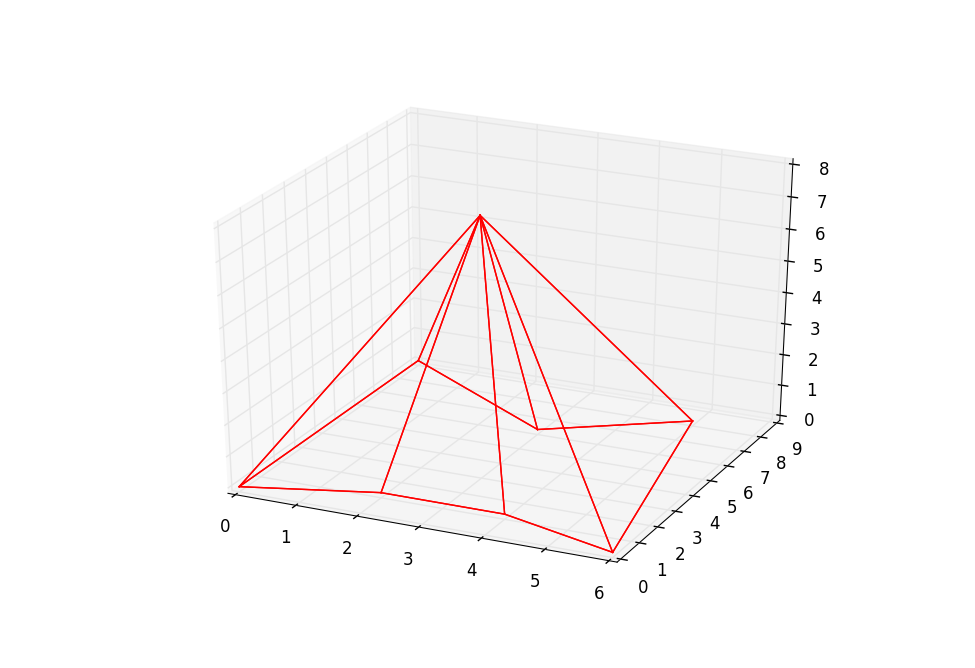
\includegraphics[scale=0.4]{Immagini/Project/matplotlibTest5.png}
\caption{Plot con Matplotlib. Un particolare elemento della Mesh che i
  VEM possono gestire.}
\end{figure}

\begin{figure}[h]
\label{img:matplotlibMesh}
\centering
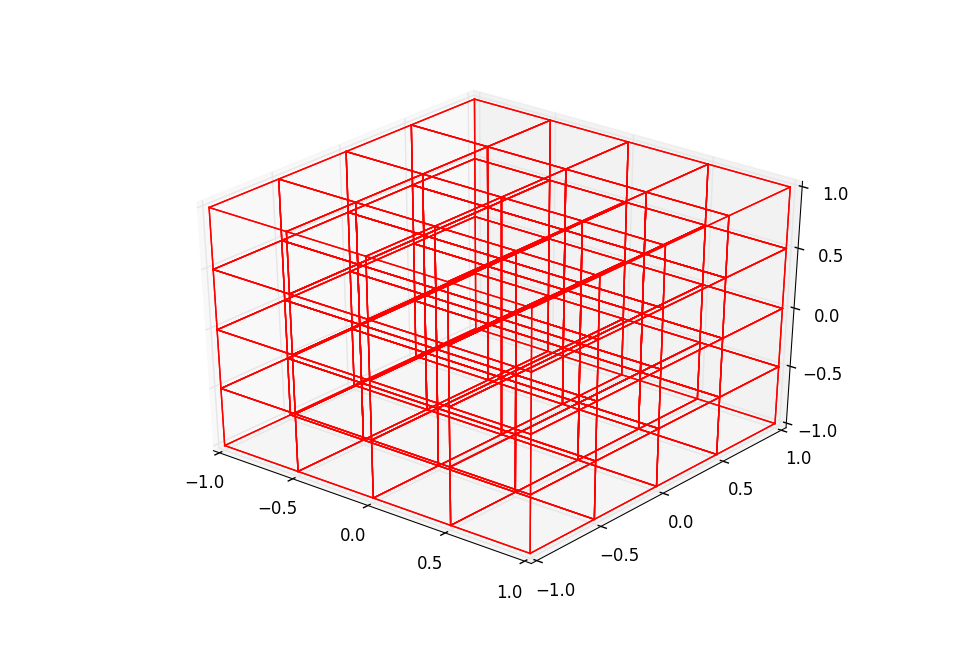
\includegraphics[scale=0.4]{Immagini/Project/matplotlibPlotMesh.png}
\caption{Plot con Matplotlib. Mesh di cubi.}
\end{figure}

\begin{figure}[h]
\label{img:mayavi2D}
\centering
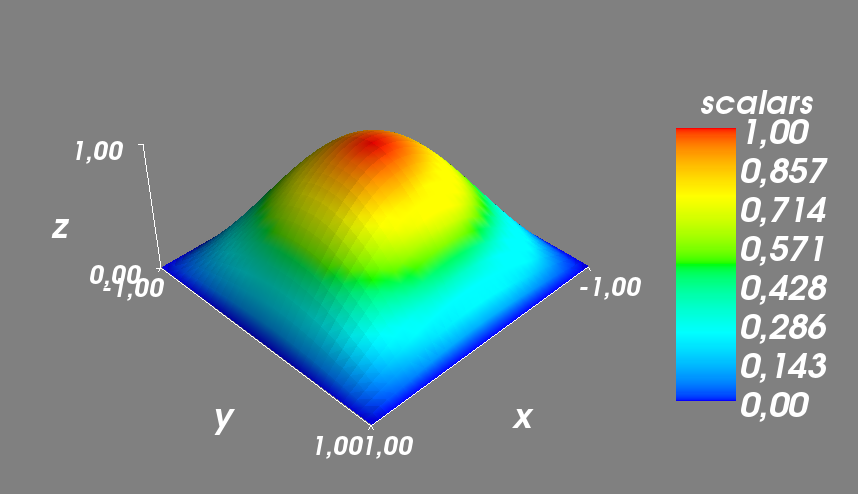
\includegraphics[scale=0.4]{Immagini/Project/mayavi2D.png}
\caption{Plot con Mayavi. Mesh di quadrati in 2D con soluzione.}
\end{figure}

\begin{figure}[h]
\label{img:matplotlibMesh}
\centering
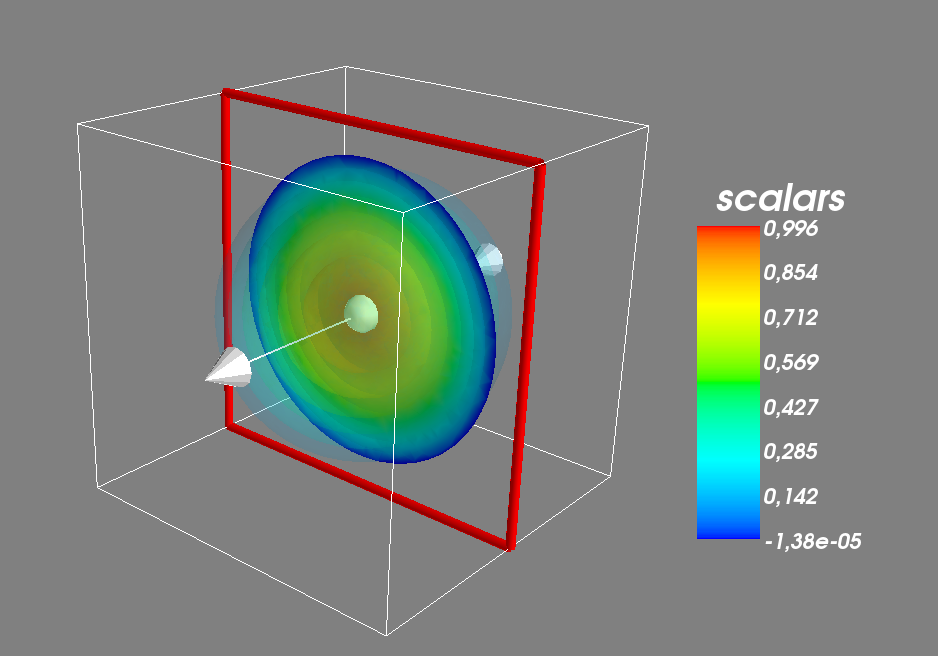
\includegraphics[scale=0.4]{Immagini/Project/mayavi3D.png}
\caption{Plot con Mayavi. Mesh di tetraedri sferica in 3D con
  soluzione in una sezione. Il piano secante pu\`o essere direzionato
  a piacere.}
\end{figure}

\begin{figure}[h]
\label{img:matplotlibMesh}
\centering
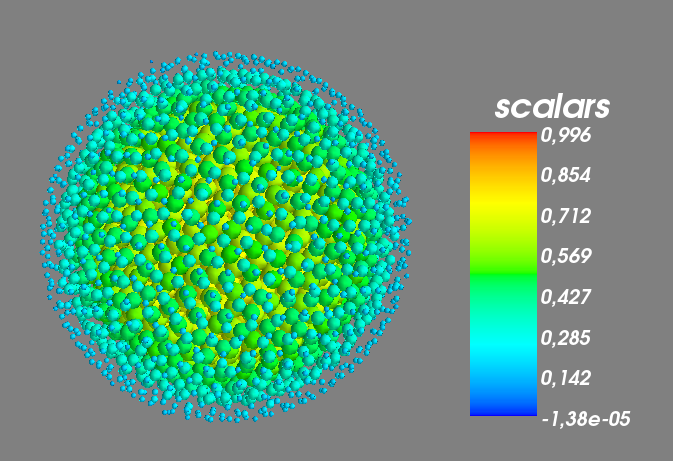
\includegraphics[scale=0.4]{Immagini/Project/mayavi3DPoints.png}
\caption{Plot con Mayavi. Mesh di tetraedri sferica in 3D con
  soluzione nei vertici}
\end{figure}

% \chapter{Un po' di fisiologia}
% \label{chap:3}

% \cite{HodgkinHuxley}
% Nel capitolo \ref{chap:1} abbiamo studiato le basi inutili di matematica. 
% Ora studieremo quelle, ancor meno utili, di fisiologia.

% Prendiamo ad esempio un cuore $\alpha$, una gamba $\beta$, 
% una mano $\mathscr M$, una faccia $\mathcal F$,
% un piede $\mathbb P$, un naso $\mathfrak N$ oppure
% un nasino $\mathsf N$ o un nasone $\nn$.
% Cosa ce ne facciamo? Nulla, appunto.
% Ma grazie alle macro si pu\`o scrivere $\MM$, $\cF$, $\P$, $\frN$, $\sfn$, $\nn$.

% Gli insiemi $\R,\Q,\N,\Z$ sono molto comodi con le macro....


% \medskip
% La bibliografia le vediamo dopo. Comunque si usa il file \emph{bibliografia.bib}
% in cui si mettono tutti i dati bibliografici; ciascuna voce avr\`a una sua label.
% Nel testo quando serve si usa poi il commando \emph{cite}: 
% ad esempio 
% %\cite{Sturm96}
% contiene tutta una matematica che non ti serve...

% Dopo aver compilato il file con \texttt{pdflatex},
% esegui il comando \texttt{bibtex} e poi \texttt{pdflatex} due volte. Alla fine compare la bibliografia aggiornata.

% Trovi il file che uso io, puoi usarlo come esempio per introdurre i testi che ti servono.



% %\appendix  % serve se vuoi creare un appendice 


% %% La bibliografia e' stata compilata e viene richiamata dal file
% %% Paper.bbl; se si vuole ricompilarla con il bibtex occorre
% %% togliere i commenti dalle due linee seguenti
% %% e alla fine aggiungere nel file Paper.bbl la riga
% %%
% %% \addcontentsline{toc}{chapter}{Bibliography}
% %%
% %% subito dopo  \begin{thebibliography}




\bibliographystyle{siam}
%\addcontentsline{toc}{chapter}{Bibliografia}
\bibliography{bibliografia}
% %\input{Paper.bbl}


% %% L'indice va stato compilato con l'istruzione
% %% 
% %% makeindex -o tesi.ind tesi.idx
% %%
% %% e viene richimato dal file tesi.ind;
% %% se si vuole ricompilarlo occorre poi 
% %% aggiungere nel file tesi.ind dopo \begin{theindex} la riga
% %% 
% %%   \addcontentsline{toc}{chapter}{Index}
% %%
% %%   
% %\input tesi.in


\end{document}









